% filepath: /Users/arihant/Documents/epita/masters_computer_science/itil/report.tex
\documentclass[12pt,a4paper]{article}
\usepackage{graphicx}
\usepackage{hyperref}
\usepackage{enumitem}
\usepackage{geometry}
\geometry{margin=1in}

\begin{document}

% Title page
\begin{titlepage}
    \centering
    \vspace*{1cm}
    % School logo
    
\includegraphics[width=0.35\textwidth]{screenshots/Epita.jpg}\par\vspace{1.5cm}
    {\LARGE\bfseries ITIL Simulation - GLPI \par}
    \vspace{0.5cm}
    {\large Report\par}
    \vspace{2cm}
    {\large\textbf{Team Members:}\par}
    \vspace{0.8cm}
    Trithikraj Doorga \\[0.3cm]
    Su Huizhe \\[0.3cm]
    Ayooluwatomi Aiyeniko \\[0.3cm]
    Arihant Jain
    \vfill
    {\large \today\par}
\end{titlepage}

% Table of contents
\tableofcontents
\newpage

\section*{Objective}
The objective of this exercise is to simulate how an IT team operates using ITIL best practices in GLPI.

\section{Part 1 - Build your CMDB}
\begin{enumerate}[label=\textbf{Step \arabic*:}, leftmargin=2cm]
    \item \textbf{Create CI:} \\
    Go to \texttt{Assets → Computers → + Add}. Create:
    \begin{itemize}
        \item WEB-SRV-Team02 (Web Server)
        \item APP-SRV-Team02 (Application Server)
        \item DB-SRV-Team02 (Database Server)
        \item ERP-SRV-Team02 (ERP Server)
    \end{itemize}
    
    \textbf{Create Screenshots:}
    
    \begin{center}
        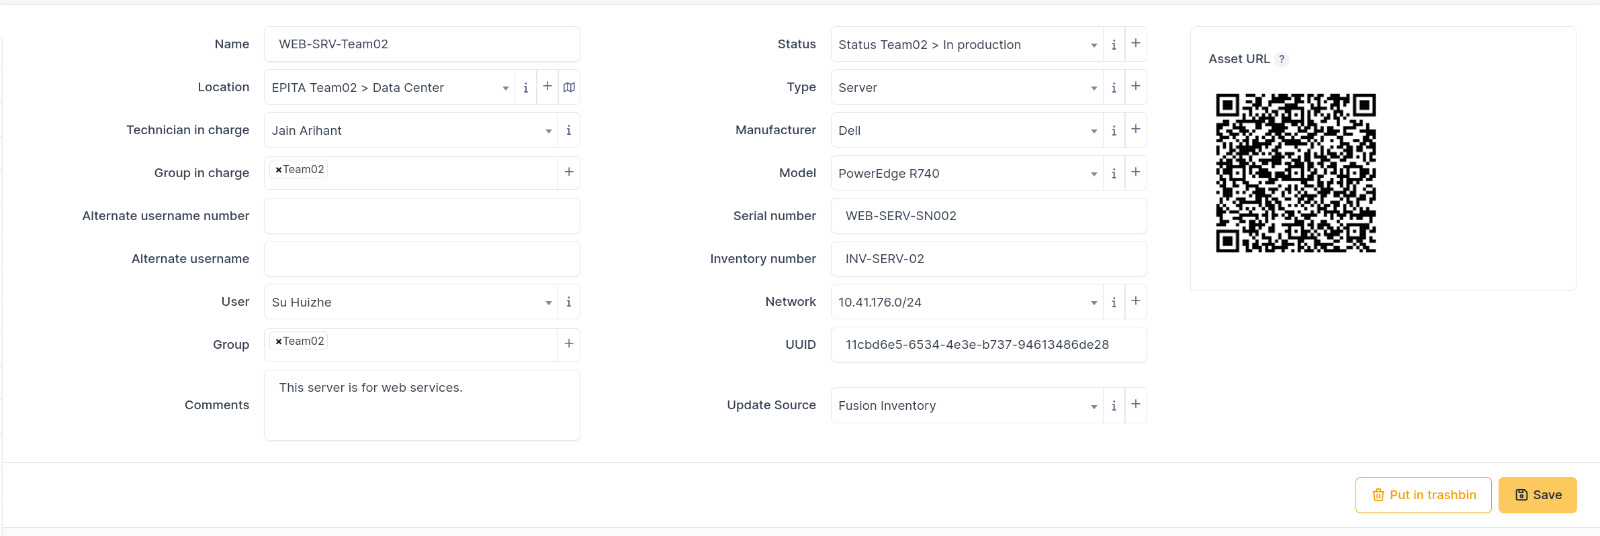
\includegraphics[width=0.85\textwidth]{screenshots/Create-WEB-SRV-Team02.jpeg} \\[0.5cm]
        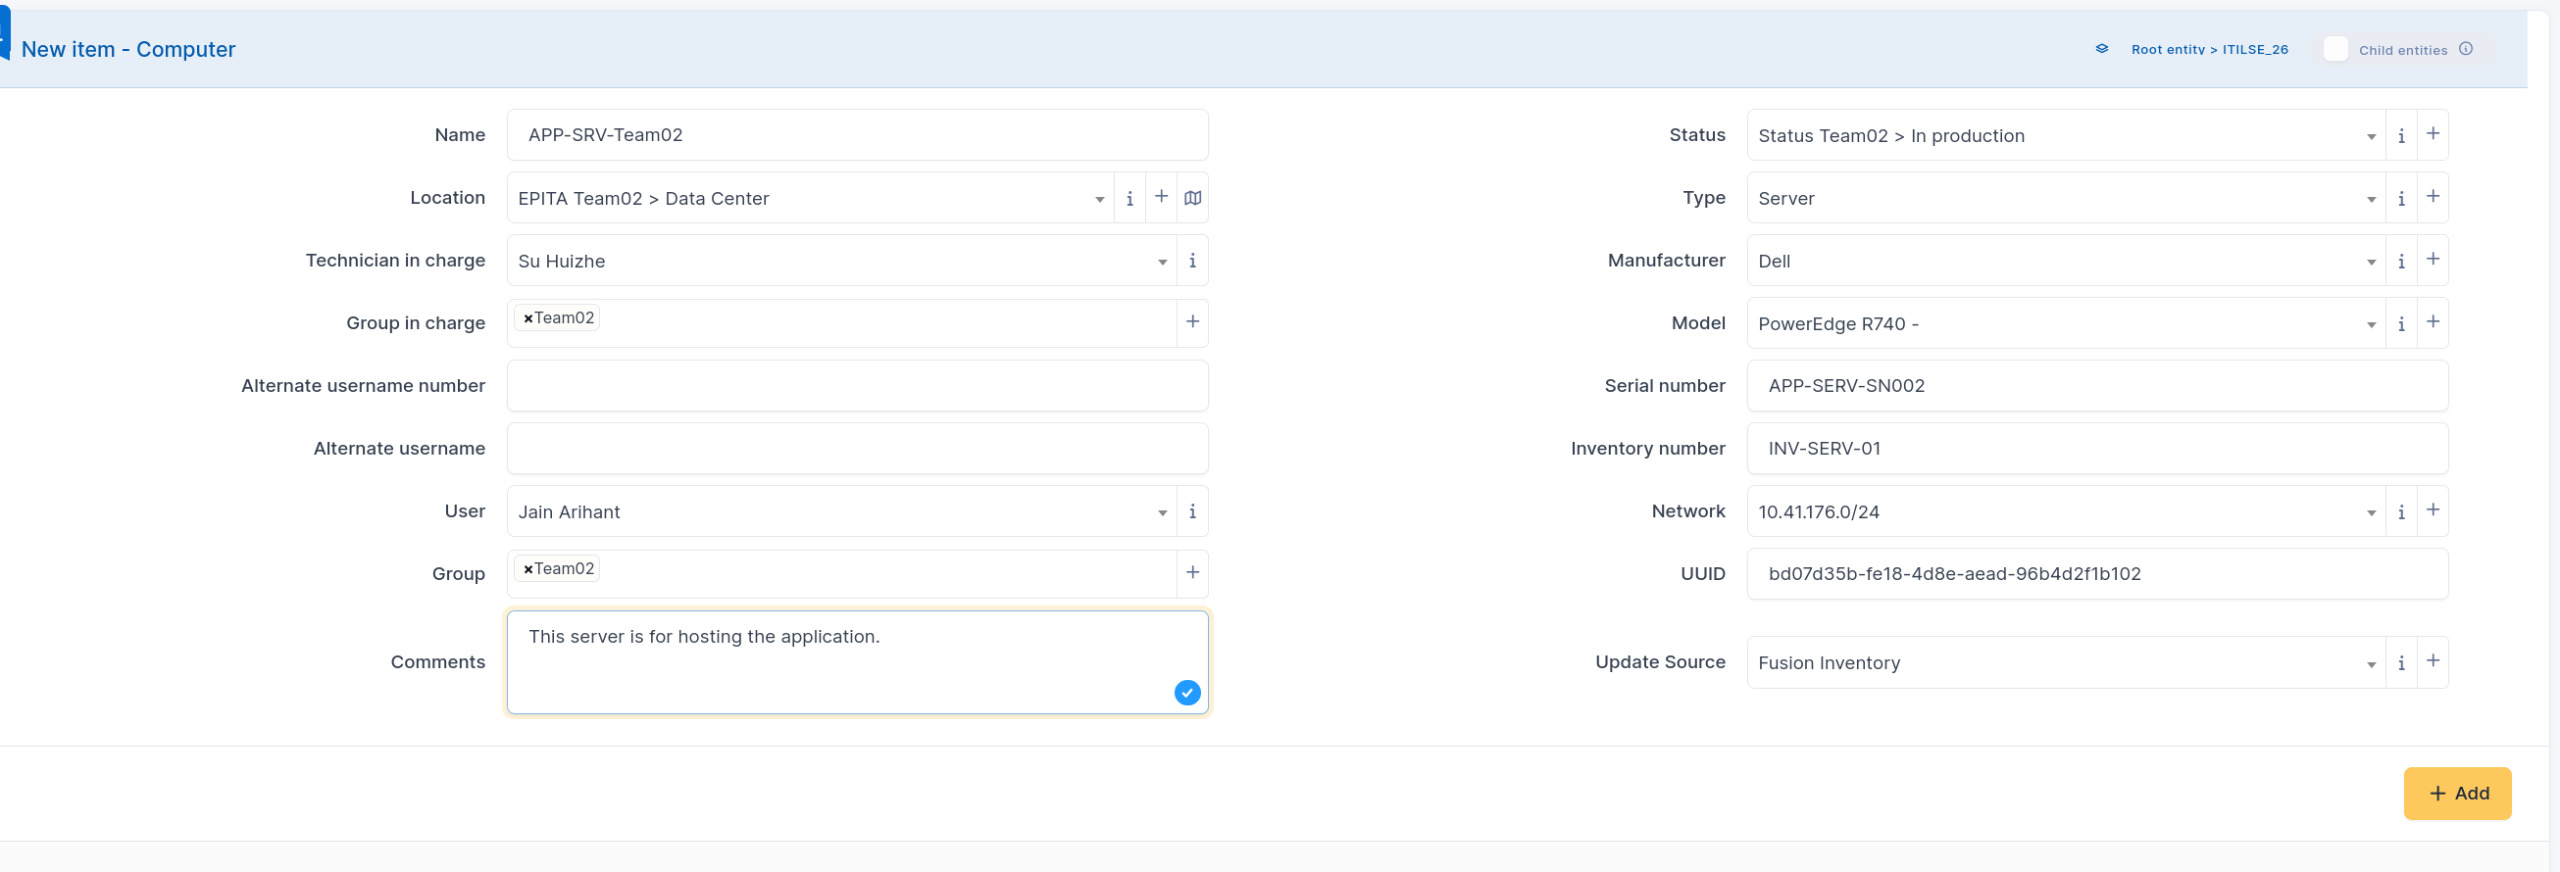
\includegraphics[width=0.85\textwidth]{screenshots/Create-APP-SRV-Team02.jpeg} \\[0.5cm]
        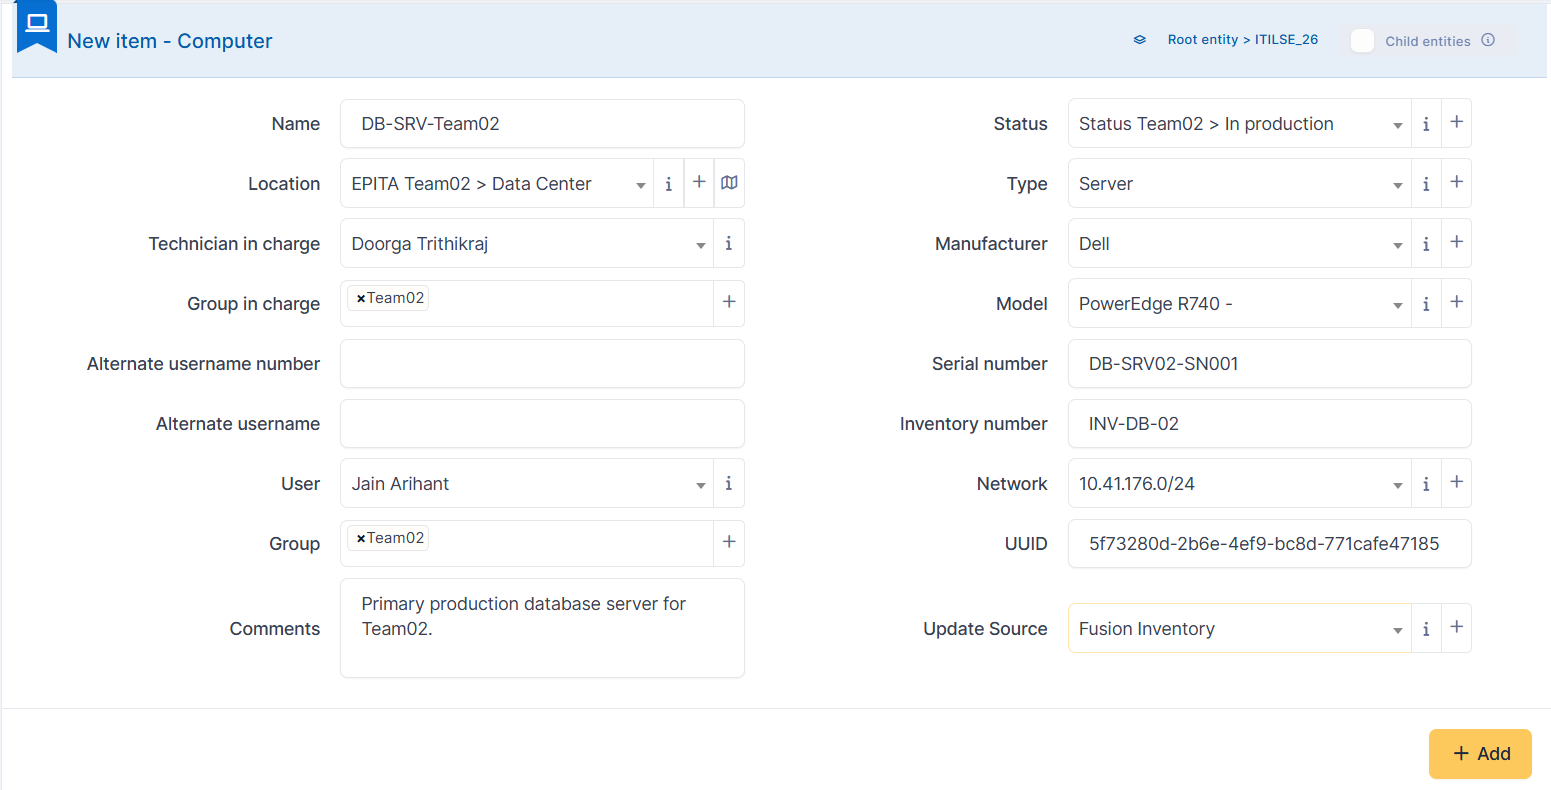
\includegraphics[width=0.85\textwidth]{screenshots/Create-DB-SRV-Team02.png} \\[0.5cm]
        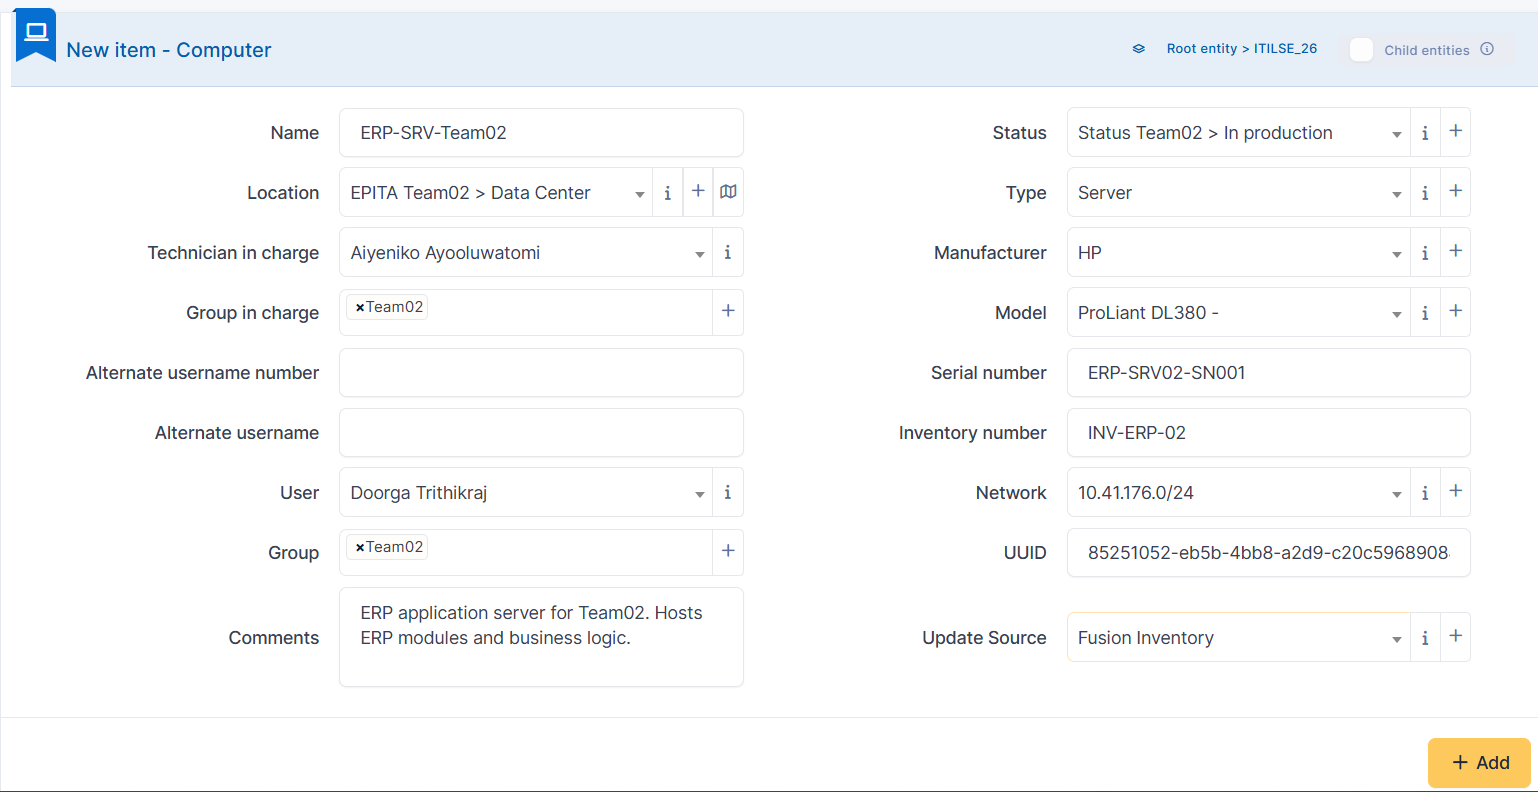
\includegraphics[width=0.85\textwidth]{screenshots/Create-ERP-SRV-Team02.png}
    \end{center}
    
    \item \textbf{Fill in CI information:}
    \begin{itemize}
        \item Name
        \item Status: In production
        \item Type: Server
        \item Location: Data Center
        \item Comments
    \end{itemize}
    \item \textbf{Define relationships:}
    \begin{itemize}
        \item WEB-SRV-Team02 \textbf{depends on} APP-SRV-Team02
        \item APP-SRV-Team02 \textbf{depends on} DB-SRV-Team02
    \end{itemize}
    Relationships are defined in GLPI by editing a CI, navigating to the \textbf{Links} or \textbf{Relationships} tab, and linking to the relevant CI with the appropriate relationship type (e.g., "Depends on").
    
    \textbf{Impact Analysis - CI Relationships:}
    \begin{center}
        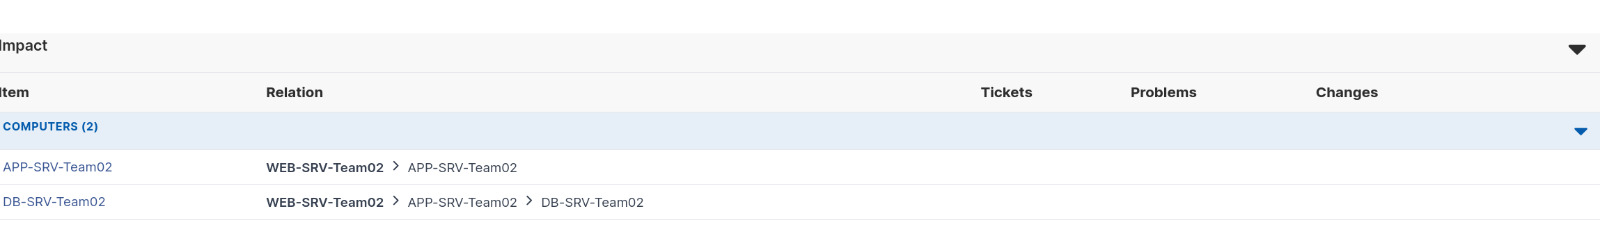
\includegraphics[width=0.9\textwidth]{screenshots/Impact-Analysis-Relation.jpeg}
    \end{center}
\end{enumerate}

\section{Part 2 - Incident Management}
\begin{enumerate}[label=\textbf{Step \arabic*:}, start=4, leftmargin=2cm]
    \item Create tickets (\texttt{Assistance → Tickets → + Add})
    
    \textbf{Create Ticket Screenshot:}
    
    \begin{center}
        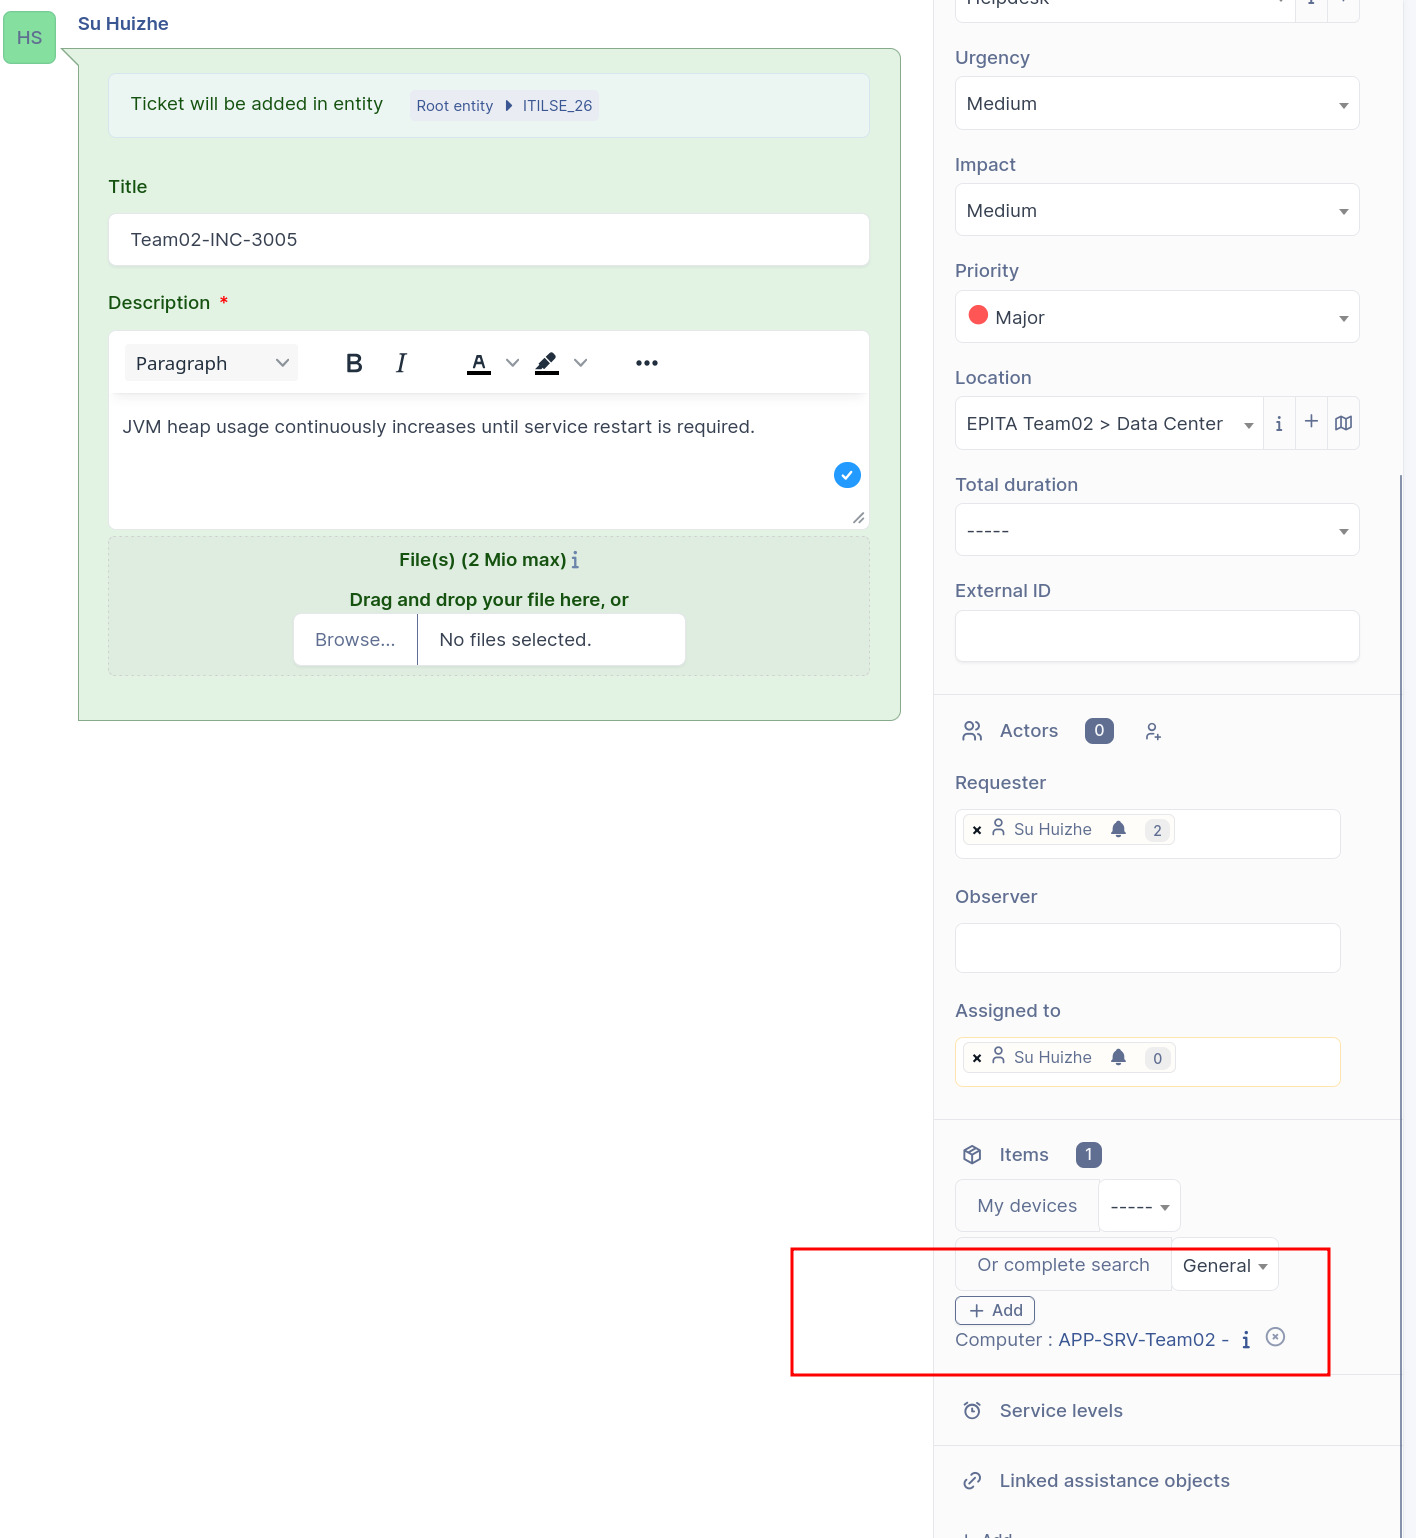
\includegraphics[width=0.85\textwidth]{screenshots/Create-Ticket.jpeg}
    \end{center}
    
    \item Link tickets to CI (\textbf{MANDATORY})
    \item Manage tickets:
    \begin{itemize}
        \item Assign
        \item Update
        \item Comment
        \item Prioritize
    \end{itemize}
    
    \textbf{Tickets List Screenshot:}
    
    \begin{center}
        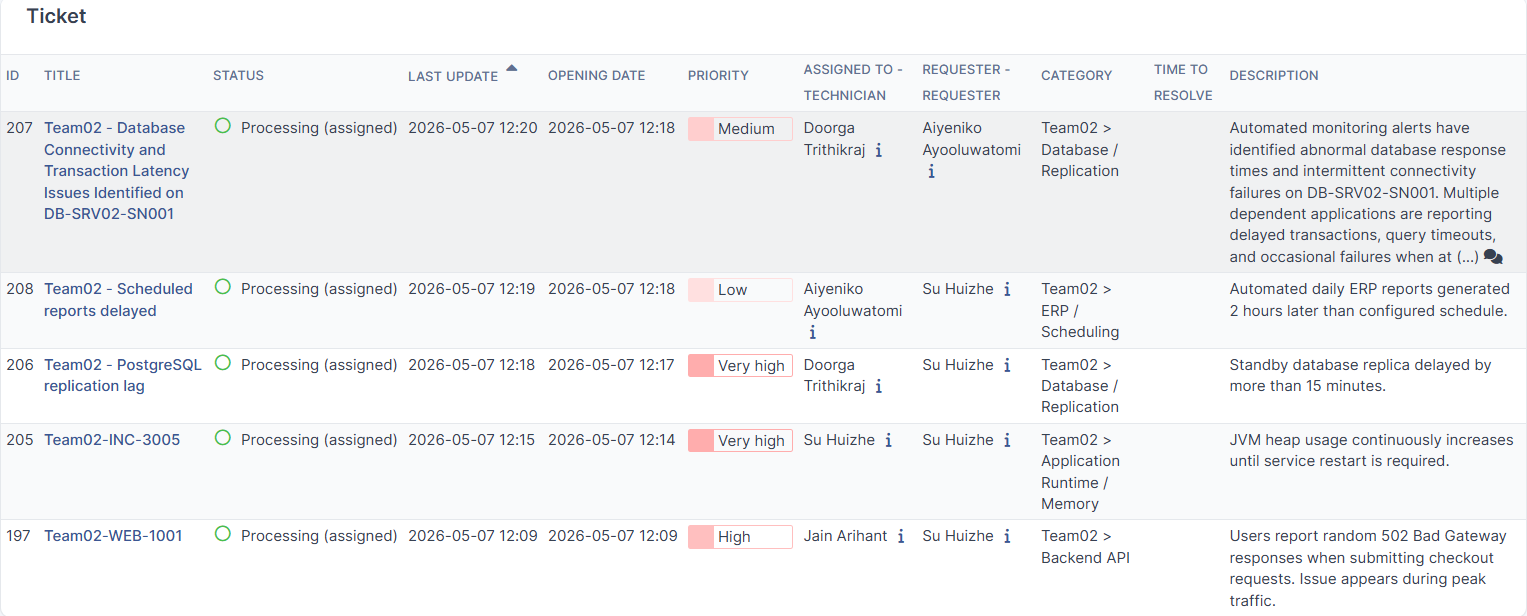
\includegraphics[width=0.9\textwidth]{screenshots/Tickets-List.png}
    \end{center}
\end{enumerate}

\section{Part 3 - Category Management}
\begin{enumerate}[label=\textbf{Step \arabic*:}, start=7, leftmargin=2cm]
    \item Create ticket category (\texttt{Administration → Ticket categories → + Add})
    
    \textbf{Create Category Screenshot:}
    
    \begin{center}
        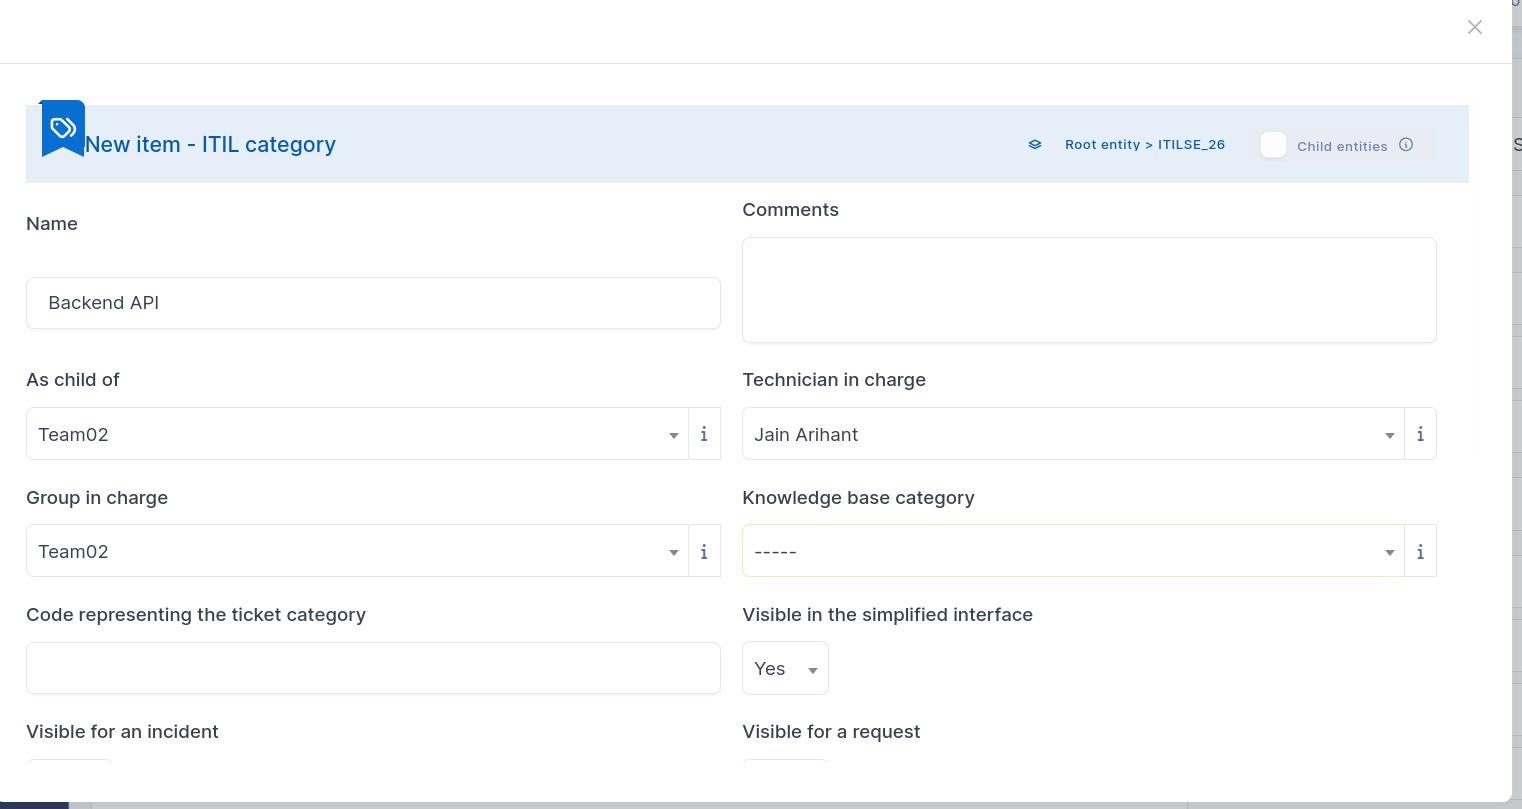
\includegraphics[width=0.85\textwidth]{screenshots/Create-Category.jpeg}
    \end{center}
\end{enumerate}

\section{Part 4 - Problem Management}
\begin{enumerate}[label=\textbf{Step \arabic*:}, start=8, leftmargin=2cm]
    \item Create a problem (\texttt{Assistance → Problems → + Add})
    \item Link incidents to the problem
    
    \textbf{Problem Screenshot:}
    
    \begin{center}
        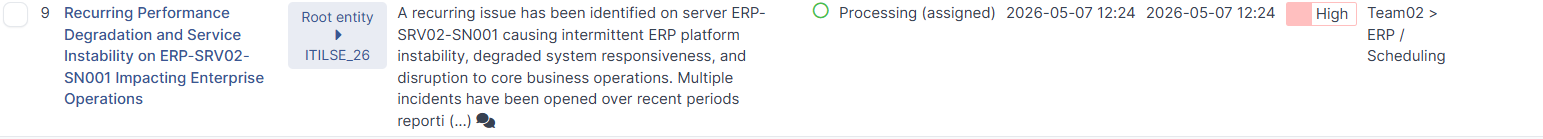
\includegraphics[width=0.85\textwidth]{screenshots/Problem.png}
    \end{center}
\end{enumerate}

\section{Part 5 - Change Management}
\begin{enumerate}[label=\textbf{Step \arabic*:}, start=10, leftmargin=2cm]
    \item Create a change request (\texttt{Assistance → Changes → + Add})
    
    \textbf{Create Change Request Screenshot:}
    
    \begin{center}
        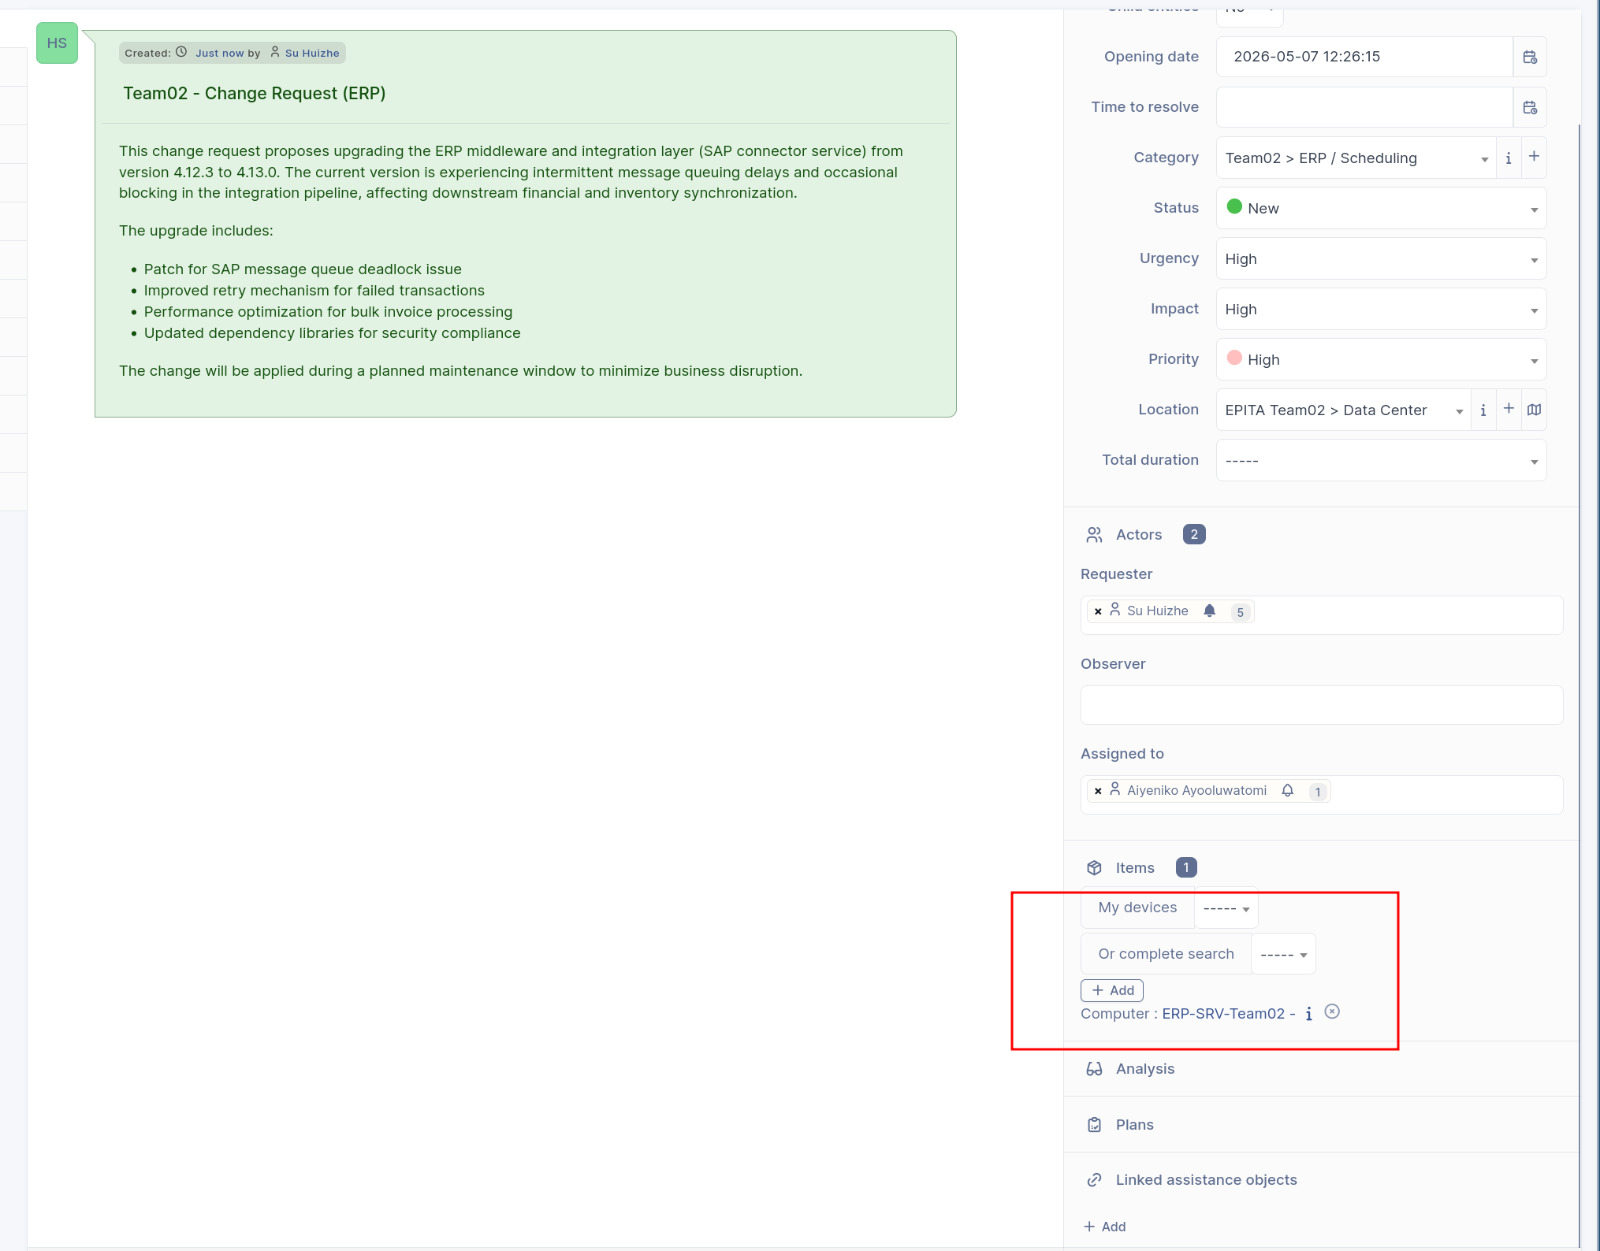
\includegraphics[width=0.85\textwidth]{screenshots/Create-Change-Request.jpeg}
    \end{center}
\end{enumerate}


\subsection*{Screenshots}
\begin{itemize}
    \item CI List - Impact Analysis:
    \begin{center}
        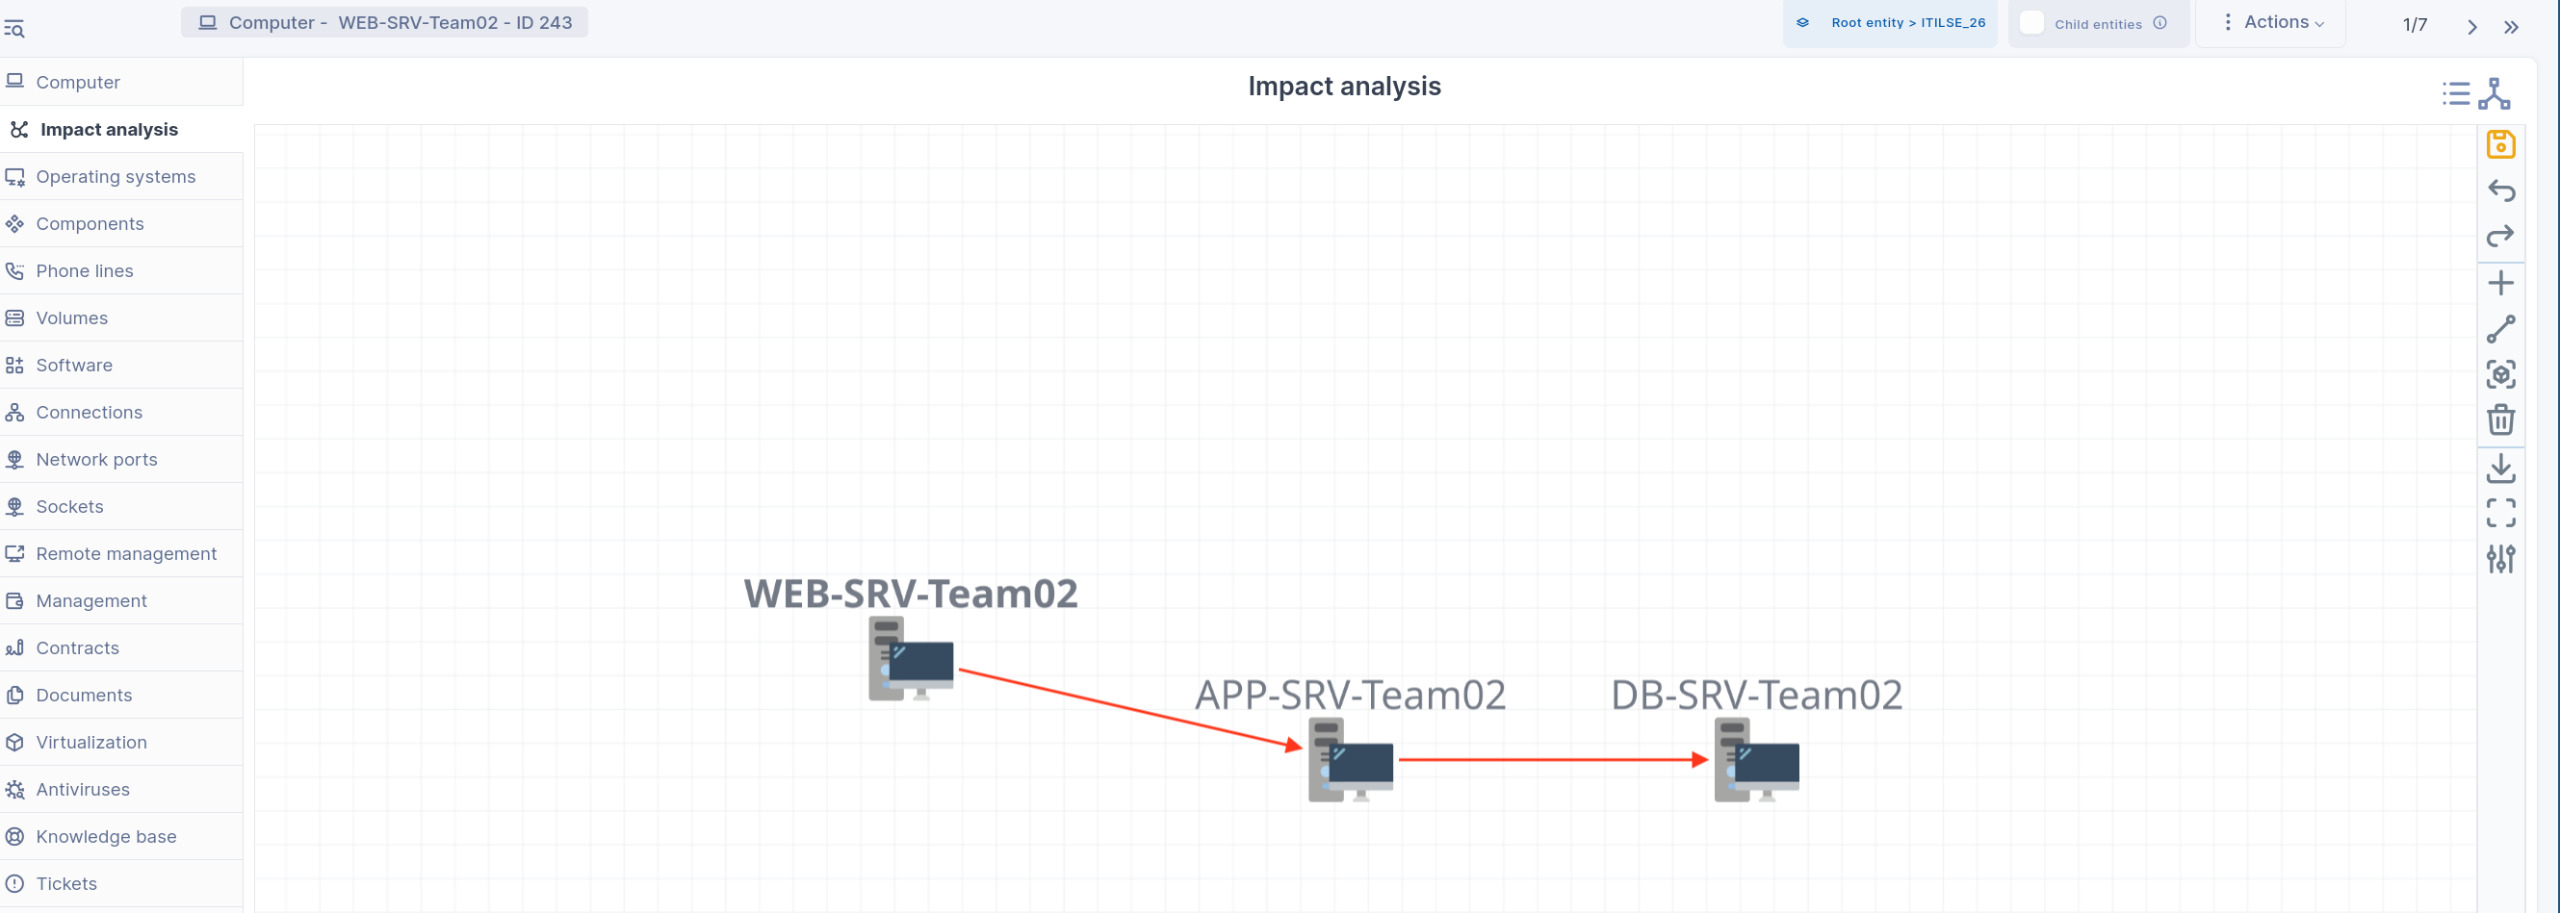
\includegraphics[width=0.75\textwidth]{screenshots/Imapct-Analysis.jpeg}
    \end{center}
    \item CI Relationships - Impact Analysis:
    \begin{center}
        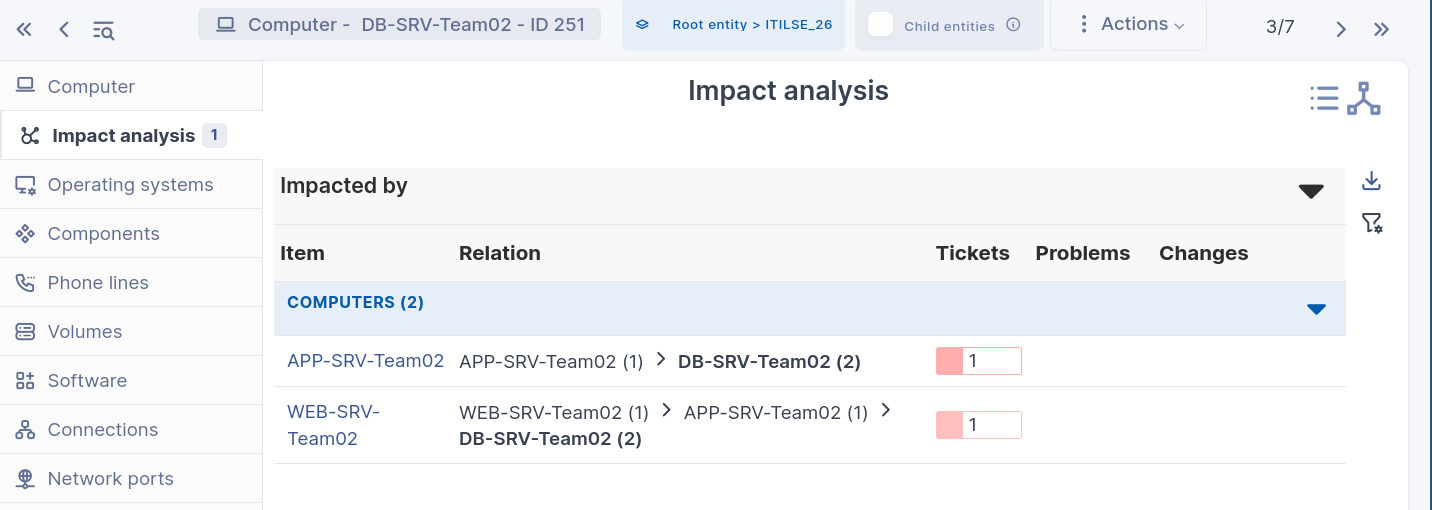
\includegraphics[width=0.75\textwidth]{screenshots/CI-Impact-Analysis.jpeg}
    \end{center}
\end{itemize}

\subsection*{Mini Dashboard}
\begin{itemize}
    \item Number of incidents: \textbf{5} (IDs: 197, 205, 206, 207, 208)
    \item Critical incidents: \textbf{2}
    \begin{itemize}
        \item ID 205 -- JVM heap memory leak (Very High)
        \item ID 206 -- PostgreSQL replication lag (Very High)
    \end{itemize}
    \item Impacted CI: \textbf{WEB-SRV-Team02, APP-SRV-Team02, DB-SRV-Team02, ERP-SRV-Team02}
    \item Root cause: \textbf{Database layer degradation on DB-SRV-Team02} (connectivity issues + replication lag). This triggered cascading failures across APP, WEB, and ERP services.
\end{itemize}

\subsection*{Short Analysis}
\begin{itemize}
    \item What happened? Database failed. All systems went down.
    \item Root cause? Database had memory leak and replication problems.
    \item Lessons learned? Database is critical. Monitor it closely.
    \item Improvements? Add database monitoring and alerts.
\end{itemize}

\end{document}